\section{New graphs and a gallery}
%<-------------------------------------------------------------------------->
% the settings of the previous sections are cancelled
\SetVertexLabel
\SetUpEdge[style = {pos=.5}]
\GraphInit[vstyle=Normal]
\subsection{Hypercubes: \tkzcname{grHypercube}}
\begin{NewMacroBox}{grHypercube}{\oarg{local options}\var{n}}
\emph{The hypercube $Q_n$: $2^n$ vertices, the words of $n$ bits, two words
being adjacent when they differ by one bit. The vertex of the word
$b_{n-1}\dots b_0$ is named \tkzname{<prefix>}$b_{n-1}\dots b_0$
(\tkzname{a000}, \tkzname{a001}\dots). The bit $k$ moves a vertex along a
vector of length \tkzname{RA}; $n=1$ to $4$ have the classic drawings.
Options: \tkzname{RA}, \tkzname{prefix}, \tkzname{Math}, \tkzname{x},
\tkzname{y}, \tkzname{rotation}.}
\end{NewMacroBox}

\begin{tkzexample}[vbox,small]
\begin{tikzpicture}
  \GraphInit[vstyle=Art]
  \grHypercube[RA=2]{3}
  \begin{scope}[xshift=7cm]
    \grHypercube[RA=1.6]{4}
  \end{scope}
  \begin{scope}[xshift=13cm]
    \grHypercube[RA=1.5,prefix=b]{5}
  \end{scope}
\end{tikzpicture}
\end{tkzexample}

\subsection{Trees: \tkzcname{grTree}}
\begin{NewMacroBox}{grTree}{\oarg{local options}\var{k}\var{depth}}
\emph{The complete $k$-ary tree; the root is at the top. The vertex $j$
($j=0,1\dots$) of the level $l$ (the root is at the level $0$) is named
\tkzname{<prefix>l;j}; its parent is \tkzname{<prefix>(l-1);(j div k)}.
Options: \tkzname{RA} (distance between two leaves), \tkzname{RB}
(distance between two levels), \tkzname{prefix}, \tkzname{Math},
\tkzname{x}, \tkzname{y}.}
\end{NewMacroBox}

\begin{tkzexample}[vbox,small]
\begin{tikzpicture}
  \GraphInit[vstyle=Art]
  \grTree[RA=.8,RB=1.4]{2}{3}
  \begin{scope}[xshift=8cm]
    \grTree[RA=.7,RB=1.6]{3}{2}
  \end{scope}
\end{tikzpicture}
\end{tkzexample}

\newpage
\subsection{A gallery}
Some graphs of graph theory, drawn with the macros of \tkzname{tkz-graph}
and \tkzname{tkz-berge}. The complete files are in the folder
\tkzname{examples} of the package.

\newpage
\subsubsection{The Petersen graph is a Kneser graph}
The vertices of the Kneser graph $K(n,k)$ are the subsets of $k$ elements of
$\{1,\dots,n\}$; two subsets are adjacent when they are disjoint. $K(5,2)$
is the Petersen graph. The edges are not given: they are computed with
\tkzcname{pgfmathtruncatemacro}, the test \tkzname{\&\&} giving $1$ for two
disjoint subsets.

\begin{tkzexample}[vbox]
\begin{tikzpicture}
  \GraphInit[vstyle=Normal]
  \tikzset{VertexStyle/.append style = {minimum size = 26pt,
                                         fill = orange!15}}
  \SetVertexMath
  \foreach \a/\b/\k in {1/2/0,3/4/1,1/5/2,2/3/3,4/5/4}
    {\Vertex[a=90+72*\k,d=4,L={\{\a,\b\}}]{\a\b}}
  \foreach \a/\b/\k in {3/5/0,2/5/1,2/4/2,1/4/3,1/3/4}
    {\Vertex[a=90+72*\k,d=2,L={\{\a,\b\}}]{\a\b}}
  \foreach \a/\b in {1/2,1/3,1/4,1/5,2/3,2/4,2/5,3/4,3/5,4/5}{%
    \foreach \c/\d in {1/2,1/3,1/4,1/5,2/3,2/4,2/5,3/4,3/5,4/5}{%
      \pgfmathtruncatemacro\ok{(\a!=\c)&&(\a!=\d)&&(\b!=\c)&&(\b!=\d)
                               &&(\a\b<\c\d)}
      \ifnum\ok=1 \Edge(\a\b)(\c\d)\fi}}
\end{tikzpicture}
\end{tkzexample}

\newpage
\subsubsection{Ramsey: $R(3,3)=6$}
Two colors for the edges of $K_5$ are enough to avoid a monochromatic
triangle (a red pentagon and a blue pentagram), but not for $K_6$: one of the
five edges from $f$ has the same color as two others, and the triangle is
red or blue. The Ramsey number $R(3,3)$ is $6$.

\begin{tkzexample}[vbox]
\begin{tikzpicture}
  \GraphInit[vstyle=Art]
  \SetGraphUnit{2.2}
  \Vertices[rotation=90]{circle}{0,1,2,3,4}
  \Edges[local,color=red,lw=1.5pt](0,1,2,3,4,0)
  \Edges[local,color=blue,lw=1.5pt](0,2,4,1,3,0)
  \Vertices[rotation=90]{circle}{0,1,2,3,4}
  \node at (0,-3) {\(K_5\) : no monochromatic triangle};
  \begin{scope}[xshift=7cm]
    \Vertices[rotation=90]{circle}{a,b,c,d,e}
    \Vertex[x=0,y=0]{f}
    \Edges[local,color=red,lw=1.5pt](a,b,c,d,e,a)
    \Edges[local,color=blue,lw=1.5pt](a,c,e,b,d,a)
    \foreach \v in {a,b}{\Edge[local,color=red,lw=1.5pt](f)(\v)}
    \foreach \v in {c,d,e}{\Edge[local,color=blue,lw=1.5pt](f)(\v)}
    \fill[red,opacity=.25] (f.center) -- (a.center) -- (b.center) -- cycle;
    \Vertices[rotation=90]{circle}{a,b,c,d,e}
    \Vertex[x=0,y=0]{f}
    \node at (0,-3) {\(K_6\) : the triangle \(f a b\) is red};
  \end{scope}
\end{tikzpicture}
\end{tkzexample}

\newpage
\subsubsection{The Moser spindle}
Seven points and eleven segments of length $1$; four colors are necessary,
so at least four colors are necessary to color the points of the plane
when two points at distance $1$ have different colors (Hadwiger--Nelson
problem). The two spindles are turned by the angle
$\theta = 2\arcsin\frac{1}{2\sqrt{3}}$ so that their tips are at distance $1$.

\begin{tkzexample}[latex=8cm,small]
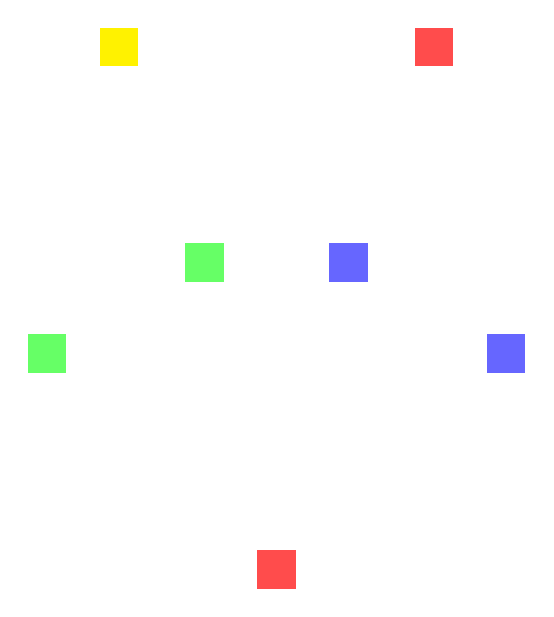
\begin{tikzpicture}[scale=4]
  \GraphInit[vstyle=Normal]
  \SetVertexNoLabel
  \tikzset{VertexStyle/.append style = {minimum size = 14pt}}
  \pgfmathsetmacro\t{2*asin(1/(2*sqrt(3)))}
  \pgfmathsetmacro\u{90-\t/2}
  \pgfmathsetmacro\w{90+\t/2}
  \tikzset{c1/.style={fill=red!70},c2/.style={fill=blue!60},
           c3/.style={fill=green!60},c4/.style={fill=yellow}}
  \coordinate (A) at (0,0);
  \coordinate (B) at (\u-30:1);  \coordinate (C) at (\u+30:1);
  \coordinate (D) at (\u:{sqrt(3)});
  \coordinate (E) at (\w-30:1);  \coordinate (F) at (\w+30:1);
  \coordinate (G) at (\w:{sqrt(3)});
  \Edges(A,B,D,C,A) \Edge(B)(C)
  \Edges(A,E,G,F,A) \Edge(E)(F)
  \Edge[local,color=red,lw=2pt](D)(G)
  \foreach \v/\c in {A/c1,B/c2,C/c3,D/c1,E/c2,F/c3,G/c4}
    {\node[VertexStyle,\c] at (\v) {};}
\end{tikzpicture}
\end{tkzexample}

\newpage
\subsubsection{Mycielski's construction}
From a graph without triangle, Mycielski's construction gives a graph
without triangle that needs one more color. Each vertex $u_i$ of $C_5$
receives a shadow $w_i$ joined to the neighbors of $u_i$, and a vertex $z$ is
joined to all the shadows: the result is the Grötzsch graph
(\tkzcname{grGrotzsch}), with $4$ colors.

\begin{tkzexample}[vbox]
\begin{tikzpicture}
  \GraphInit[vstyle=Normal]
  \SetVertexMath
  \tikzset{VertexStyle/.append style = {minimum size = 20pt}}
  \foreach \i/\c in {0/red!50,1/blue!40,2/red!50,3/blue!40,4/green!50}{%
    \begin{scope}[VertexStyle/.append style = {fill = \c}]
      \Vertex[a=90+72*\i,d=4.5,L={u_{\i}}]{u\i}
      \Vertex[a=90+72*\i,d=2.2,L={w_{\i}}]{w\i}
    \end{scope}}
  \begin{scope}[VertexStyle/.append style = {fill = yellow}]
    \Vertex[x=0,y=0,L=z]{z}
  \end{scope}
  \Edges[lw=1.5pt](u0,u1,u2,u3,u4,u0)
  \foreach \i in {0,...,4}{%
    \pgfmathtruncatemacro\p{mod(\i+4,5)}
    \pgfmathtruncatemacro\n{mod(\i+1,5)}
    \Edge[color=gray](w\i)(u\p)
    \Edge[color=gray](w\i)(u\n)
    \Edge[color=orange,style={dashed}](z)(w\i)}
\end{tikzpicture}
\end{tkzexample}

\newpage
\subsubsection{The de Bruijn graph $B(2,3)$}
The vertices are the words of three bits, and there is an arc
$abc\to bcd$ labelled $d$. Each vertex has two arcs in and two arcs out:
there is an Eulerian cycle. The bits read in the order of the numbers give a
de Bruijn sequence: each word of four bits appears once in it. This example
needs \tkzname{lualatex} and the option \tkzname{lua}
(\tkzcname{tkzGraphEuler}).

\begin{tkzexample}[vbox]
\begin{tikzpicture}[scale=.8]
  \GraphInit[vstyle=Normal]
  \tikzset{VertexStyle/.append style = {minimum size = 24pt,
                                         fill = cyan!15}}
  \tikzset{LabelStyle/.style = {fill = white, font = \footnotesize,
                                inner sep = 1pt}}
  \tikzset{EulerNumberStyle/.style = {circle, fill = red!80!black,
           text = white, inner sep = 1pt, font = \tiny\bfseries}}
  \Vertex[x=0,y=0]{000}
  \Vertex[x=3,y=2]{001}    \Vertex[x=3,y=-2]{100}
  \Vertex[x=5,y=0]{010}    \Vertex[x=8,y=0]{101}
  \Vertex[x=10,y=2]{011}   \Vertex[x=10,y=-2]{110}
  \Vertex[x=13,y=0]{111}
  \Loop[dir=WE,dist=2cm,style={->},label=0](000)
  \Loop[dir=EA,dist=2cm,style={->},label=1](111)
  \Edge[->,label=1](000)(001)
  \Edge[->,label=0](001)(010)
  \Edge[->,label=1](001)(011)
  \Edge[->,label=0](010)(100)
  \Edge[->,label=1,style={bend left=20}](010)(101)
  \Edge[->,label=0,style={bend left=20}](101)(010)
  \Edge[->,label=1](101)(011)
  \Edge[->,label=0](011)(110)
  \Edge[->,label=1](011)(111)
  \Edge[->,label=0](100)(000)
  \Edge[->,label=1](100)(001)
  \Edge[->,label=0](110)(100)
  \Edge[->,label=1](110)(101)
  \Edge[->,label=0](111)(110)
  \tkzGraphEuler[numbers,pos=.3,start=000]
\end{tikzpicture}
\end{tkzexample}

\newpage
\subsubsection{The Paley graph $P_{13}$}
In $P_{13}$, $i$ and $j$ are adjacent when $i-j$ is a square modulo $13$
($\pm1$, $\pm3$, $\pm4$): it is the circulant graph \tkzcname{grCirculant}
with $1,3,4$. Its complement ($2,5,6$) is isomorphic to it: the edges of
$K_{13}$ are split into two copies of the same graph.

\begin{tkzexample}[vbox]
\begin{tikzpicture}[scale=.7]
  \GraphInit[vstyle=Art]
  \SetUpEdge[color=red!80!black,lw=1pt]
  \grCirculant[RA=3]{13}{1,3,4}
  \begin{scope}[xshift=7.5cm]
    \SetUpEdge[color=blue!70!black,lw=1pt]
    \grCirculant[RA=3]{13}{2,5,6}
  \end{scope}
  \begin{scope}[xshift=15cm]
    \SetUpEdge[color=red!80!black,lw=.8pt]
    \grCirculant[RA=3]{13}{1,3,4}
    \SetUpEdge[color=blue!70!black,lw=.8pt]
    \grCirculant[RA=3]{13}{2,5,6}
  \end{scope}
  \node at (0,-4)    {\(P_{13}\)};
  \node at (7.5,-4)  {\(\overline{P_{13}}\simeq P_{13}\)};
  \node at (15,-4)   {\(K_{13}=P_{13}\cup\overline{P_{13}}\)};
\end{tikzpicture}
\end{tkzexample}

\newpage
\subsubsection{The hypercube $Q_4$ and the subsets of a set}
$Q_4$ drawn as the Hasse diagram of the subsets of $\{a,b,c,d\}$: an edge
joins two subsets when one is obtained by adding an element to the other;
its color gives this element. Compare with \tkzcname{grHypercube}.

\begin{tkzexample}[vbox]
\begin{tikzpicture}[xscale=1.4,yscale=2.2]
  \GraphInit[vstyle=Normal]
  \SetVertexMath
  \tikzset{VertexStyle/.append style = {rectangle, rounded corners,
            minimum size = 18pt, fill = white}}
  \foreach \n/\x/\y/\l in {
     0/0/0/{\emptyset},
     a/-3/1/{\{a\}}, b/-1/1/{\{b\}}, c/1/1/{\{c\}}, d/3/1/{\{d\}},
     ab/-5/2/{\{a,b\}}, ac/-3/2/{\{a,c\}}, ad/-1/2/{\{a,d\}},
     bc/1/2/{\{b,c\}},  bd/3/2/{\{b,d\}},  cd/5/2/{\{c,d\}},
     abc/-3/3/{\{a,b,c\}}, abd/-1/3/{\{a,b,d\}},
     acd/1/3/{\{a,c,d\}},  bcd/3/3/{\{b,c,d\}},
     abcd/0/4/{\{a,b,c,d\}}}
   {\Vertex[x=\x,y=\y,L=\l]{\n}}
  \foreach \s/\t/\c in {
    0/a/red, 0/b/blue, 0/c/green!60!black, 0/d/orange, a/ab/blue,
    a/ac/green!60!black, a/ad/orange, b/ab/red, b/bc/green!60!black,
    b/bd/orange, c/ac/red, c/bc/blue, c/cd/orange, d/ad/red,
    d/bd/blue, d/cd/green!60!black, ab/abc/green!60!black,
    ab/abd/orange, ac/abc/blue, ac/acd/orange, ad/abd/blue,
    ad/acd/green!60!black, bc/abc/red, bc/bcd/orange, bd/abd/red,
    bd/bcd/green!60!black, cd/acd/red, cd/bcd/blue, abc/abcd/orange,
    abd/abcd/green!60!black, acd/abcd/blue, bcd/abcd/red}
    {\Edge[local,color=\c,lw=1.2pt](\s)(\t)}
  \foreach \n/\x/\y/\l in {
     0/0/0/{\emptyset},
     a/-3/1/{\{a\}}, b/-1/1/{\{b\}}, c/1/1/{\{c\}}, d/3/1/{\{d\}},
     ab/-5/2/{\{a,b\}}, ac/-3/2/{\{a,c\}}, ad/-1/2/{\{a,d\}},
     bc/1/2/{\{b,c\}},  bd/3/2/{\{b,d\}},  cd/5/2/{\{c,d\}},
     abc/-3/3/{\{a,b,c\}}, abd/-1/3/{\{a,b,d\}},
     acd/1/3/{\{a,c,d\}},  bcd/3/3/{\{b,c,d\}},
     abcd/0/4/{\{a,b,c,d\}}}
   {\Vertex[x=\x,y=\y,L=\l]{\n}}
\end{tikzpicture}
\end{tkzexample}

\newpage
\subsubsection{The Tower of Hanoi}
The 81 states of the Tower of Hanoi with 4 discs; two states are adjacent
when one move goes from one to the other. This graph is the Sierpiński
graph $S(4,3)$: a vertex $d_1d_2d_3d_4$ is placed at the sum of the corners
$c(d_k)$ multiplied by $L^{4-k}$, and $s\,i\,j\dots j$ is adjacent to
$s\,j\,i\dots i$. The colors give the size of the disc moved. The bottom side,
from $0000$ to $2222$, is an optimal solution (15 moves): the words of
$\{0,2\}^4$ in the order of the binary numbers.

\begin{tkzexample}[vbox]
\begin{tikzpicture}[scale=.55]
  \GraphInit[vstyle=Art]
  \SetVertexNoLabel
  \tikzset{VertexStyle/.append style = {minimum size = 5pt}}
  \def\L{2.35}
  \def\cx{{0,0.5,1}}\def\cy{{0,0.866,0}}
  \foreach \a in {0,1,2}{\foreach \b in {0,1,2}{%
  \foreach \c in {0,1,2}{\foreach \d in {0,1,2}{%
    \pgfmathsetmacro\x{\cx[\a]*\L^3+\cx[\b]*\L^2+\cx[\c]*\L+\cx[\d]}
    \pgfmathsetmacro\y{\cy[\a]*\L^3+\cy[\b]*\L^2+\cy[\c]*\L+\cy[\d]}
    \Vertex[x=\x,y=\y]{\a\b\c\d}}}}}
  \foreach \i/\j in {0/1,0/2,1/2}{%
    \foreach \a in {0,1,2}{\foreach \b in {0,1,2}{\foreach \c in {0,1,2}{%
      \Edge[local,color=gray,lw=.6pt](\a\b\c\i)(\a\b\c\j)}}}
    \foreach \a in {0,1,2}{\foreach \b in {0,1,2}{%
      \Edge[local,color=blue,lw=.8pt](\a\b\i\j)(\a\b\j\i)}}
    \foreach \a in {0,1,2}{%
      \Edge[local,color=green!60!black,lw=1pt](\a\i\j\j)(\a\j\i\i)}
    \Edge[local,color=orange,lw=1.2pt](\i\j\j\j)(\j\i\i\i)}
  \tkzHighlightPath[color=red,lw=2.5pt,style={opacity=.6}]%
    {0000,0002,0020,0022,0200,0202,0220,0222,
     2000,2002,2020,2022,2200,2202,2220,2222}
\end{tikzpicture}
\end{tkzexample}

\newpage
\subsubsection{The Hoffman--Singleton graph}
50 vertices, 175 edges, 7-regular, girth 5: a Moore graph. Robertson's
construction: five pentagons $P_h$, five pentagrams $Q_i$, and $P_{hj}$ is
adjacent to $Q_{ik}$ when $k=hi+j \pmod 5$. The color of an edge gives $h$.

\begin{tkzexample}[vbox]
\begin{tikzpicture}
  \GraphInit[vstyle=Art]
  \SetVertexNoLabel
  \tikzset{VertexStyle/.append style = {minimum size = 6pt}}
  \def\R{6}\def\r{.9}
  \foreach \h in {0,...,4}{\foreach \j in {0,...,4}{%
    \pgfmathsetmacro\x{\R*cos(72*\h+90)+\r*cos(72*\j+90)}
    \pgfmathsetmacro\y{\R*sin(72*\h+90)+\r*sin(72*\j+90)}
    \Vertex[x=\x,y=\y]{P\h\j}
    \pgfmathsetmacro\x{(\R-2.2)*cos(72*\h+126)+\r*cos(72*\j+90)}
    \pgfmathsetmacro\y{(\R-2.2)*sin(72*\h+126)+\r*sin(72*\j+90)}
    \Vertex[x=\x,y=\y]{Q\h\j}}}
  \foreach \h/\c in {0/red,1/orange,2/green!60!black,3/blue,4/violet}{%
    \foreach \i in {0,...,4}{\foreach \j in {0,...,4}{%
      \pgfmathtruncatemacro\k{mod(\h*\i+\j,5)}
      \Edge[local,color=\c!70,lw=.4pt](P\h\j)(Q\i\k)}}}
  \foreach \h in {0,...,4}{%
    \Edges[local,lw=1.2pt](P\h0,P\h1,P\h2,P\h3,P\h4,P\h0)
    \Edges[local,lw=1.2pt](Q\h0,Q\h2,Q\h4,Q\h1,Q\h3,Q\h0)}
  \foreach \h in {0,...,4}{\foreach \j in {0,...,4}{%
    \Vertex[Node]{P\h\j}\Vertex[Node]{Q\h\j}}}
\end{tikzpicture}
\end{tkzexample}

\newpage
\subsubsection{The mystic rose}
The complete graph $K_{24}$; the color of an edge (hue of the model
\tkzname{hsb}) gives the distance between its ends along the circle.

\begin{tkzexample}[vbox]
\begin{tikzpicture}
  \GraphInit[vstyle=Art]
  \SetVertexNoLabel
  \tikzset{VertexStyle/.append style = {minimum size = 6pt}}
  \grEmptyCycle[RA=6]{24}
  \foreach \d in {1,...,12}{%
    \pgfmathsetmacro\hue{(\d-1)/12}
    \definecolor{h}{hsb}{\hue,0.9,0.85}
    \colorlet{c}[rgb]{h}
    \pgfmathtruncatemacro\m{\d==12 ? 11 : 23}
    \foreach \i in {0,...,\m}{%
      \pgfmathtruncatemacro\j{mod(\i+\d,24)}
      \Edge[local,color=c,lw=.5pt](a\i)(a\j)}}
  \grEmptyCycle[RA=6]{24}
\end{tikzpicture}
\end{tkzexample}

\newpage
\subsubsection{The Coxeter graph}
28 vertices, 42 edges, cubic, girth 7, not Hamiltonian. Three 7-cycles
$a$ (step 1), $b$ (step 2) and $c$ (step 3) on the same circle, and $d_i$
joined to $a_i$, $b_i$ and $c_i$.

\begin{tkzexample}[vbox]
\begin{tikzpicture}
  \GraphInit[vstyle=Art]
  \SetVertexNoLabel
  \tikzset{VertexStyle/.append style = {minimum size = 8pt}}
  \foreach \i in {0,...,6}{%
    \pgfmathsetmacro\t{90+360*\i/7}
    \Vertex[a=\t,d=5]{a\i}
    \Vertex[a=\t+360/21,d=5]{b\i}
    \Vertex[a=\t-360/21,d=5]{c\i}
    \Vertex[a=\t,d=2.2]{d\i}}
  \foreach \i in {0,...,6}{%
    \pgfmathtruncatemacro\p{mod(\i+1,7)}
    \pgfmathtruncatemacro\q{mod(\i+2,7)}
    \pgfmathtruncatemacro\r{mod(\i+3,7)}
    \Edge[local,color=red,lw=1.2pt](a\i)(a\p)
    \Edge[local,color=blue,lw=1.2pt](b\i)(b\q)
    \Edge[local,color=green!60!black,lw=1.2pt](c\i)(c\r)
    \foreach \v in {a,b,c}{\Edge[local,color=gray,lw=1pt](d\i)(\v\i)}}
  \foreach \i in {0,...,6}{\foreach \v in {a,b,c,d}{\Vertex[Node]{\v\i}}}
\end{tikzpicture}
\end{tkzexample}

\endinput
